% llm-matmeta — presentation (Beamer, 16:9)
% Build: xelatex slides.tex   (twice)
\documentclass[aspectratio=169,10pt,t]{beamer}

% ---------------------------------------------------------------- fonts
\usefonttheme{professionalfonts}
\usepackage{mathpazo}
\usepackage[no-math]{fontspec}
\setsansfont{FiraSans}[Ligatures=TeX,Extension=.ttf,UprightFont=*-Light,BoldFont=*-Medium,ItalicFont=*-LightItalic,BoldItalicFont=*-MediumItalic]
\newfontfamily\fsemi{FiraSans-SemiBold.ttf}[Ligatures=TeX]
\newfontfamily\fbook{FiraSans}[Ligatures=TeX,Extension=.ttf,UprightFont=*-Regular,BoldFont=*-SemiBold,ItalicFont=*-Italic]
\newfontfamily\fthin{FiraSans-ExtraLight.ttf}[Ligatures=TeX]
\setmonofont{DejaVu Sans Mono}[Scale=0.80]

\usepackage{amsmath,amssymb,mathtools}
\usepackage{tikz}
\usetikzlibrary{positioning,arrows.meta,calc,fit,backgrounds}
\usepackage{booktabs,tabularx,array}
\usepackage[most]{tcolorbox}
\usepackage{listings}
\usepackage{appendixnumberbeamer}
\usepackage{ragged2e}

% ---------------------------------------------------------------- palette (same as the formalism)
\definecolor{ink}{HTML}{1F2A37}
\definecolor{accent}{HTML}{1D4E89}
\definecolor{accentdark}{HTML}{143A68}
\definecolor{parser}{HTML}{1B7F5B}
\definecolor{llm}{HTML}{C2571A}
\definecolor{evid}{HTML}{6B46C1}
\definecolor{quote}{HTML}{B4237A}
\definecolor{merged}{HTML}{1D4E89}
\definecolor{soft}{HTML}{F3F6FA}
\definecolor{rule}{HTML}{C9D3DF}
\definecolor{muted}{HTML}{6B7785}
\definecolor{good}{HTML}{1B7F5B}
\definecolor{bad}{HTML}{B42318}

% ---------------------------------------------------------------- notation
\newcommand{\rP}{\textcolor{parser}{r_{\mathrm{P}}}}
\newcommand{\rM}{\textcolor{llm}{r_{\mathrm{M}}}}
\newcommand{\rF}{\textcolor{merged}{r}}
\newcommand{\Ev}{\textcolor{evid}{\mathcal{E}}}
\newcommand{\Src}{\textcolor{evid}{T}}
\newcommand{\Qt}{\textcolor{quote}{q}}
\newcommand{\Prov}{\textcolor{merged}{\pi}}
\newcommand{\Conf}{\textcolor{merged}{\mathcal{C}}}
\newcommand{\Model}{\textcolor{llm}{\mathsf{M}}}
\newcommand{\Pars}{\textcolor{parser}{\mathsf{P}}}
\newcommand{\Merge}{\mathbin{\textcolor{merged}{\oplus}}}
\newcommand{\Over}{\mathbin{\textcolor{parser}{\lhd}}}
\newcommand{\agree}{\mathrel{\textcolor{merged}{\simeq}}}
\newcommand{\nagree}{\mathrel{\textcolor{bad}{\not\simeq}}}
\newcommand{\Fset}{\mathbb{F}}
\newcommand{\Vset}{\mathbb{V}}
\newcommand{\nil}{\varnothing}
\newcommand{\valid}{\mathsf{V}}
\newcommand{\Kop}{\textcolor{evid}{K}}
\newcommand{\lam}{\textcolor{quote}{\lambda}}
\newcommand{\norm}{\nu}
\newcommand{\code}[1]{\texttt{#1}}
\newcommand{\vtag}[1]{\texttt{#1}}
\newcommand{\hl}[2]{\textcolor{#1}{\fbook #2}}
\newcommand{\muted}[1]{\textcolor{muted}{#1}}
\DeclareMathOperator{\Nums}{\mathcal{N}}

% ---------------------------------------------------------------- theme
\setbeamercolor{normal text}{fg=ink,bg=white}
\setbeamercolor{structure}{fg=accent}
\setbeamercolor{alerted text}{fg=llm}
\setbeamercolor{itemize item}{fg=accent}
\setbeamercolor{itemize subitem}{fg=muted}
\setbeamercolor{enumerate item}{fg=accent}
\setbeamertemplate{navigation symbols}{}
\setbeamertemplate{itemize item}{\raisebox{0.18ex}{\tikz\fill[accent] (0,0) rectangle (0.75ex,0.75ex);}}
\setbeamertemplate{itemize subitem}{\textcolor{muted}{--}}
\setbeamertemplate{enumerate item}{\fsemi\color{accent}\insertenumlabel.}
\setlength{\leftmargini}{1.3em}
\setbeamersize{text margin left=10mm,text margin right=10mm}
\setbeamerfont{frametitle}{family=\fsemi,size=\Large}
\setbeamerfont{framesubtitle}{family=\fbook,size=\small}

\setbeamertemplate{frametitle}{%
  \vspace*{3.5mm}%
  \ifx\insertsectionhead\@empty\else
    {\fbook\scriptsize\color{muted}\MakeUppercase{\insertsectionhead}}\par\vspace{0.5mm}%
  \fi
  {\usebeamerfont{frametitle}\color{accent}\insertframetitle}\par
  \ifx\insertframesubtitle\@empty\else{\usebeamerfont{framesubtitle}\color{muted}\insertframesubtitle\par}\fi
  \vspace{1.2mm}{\color{rule}\rule{\textwidth}{0.5pt}}\vspace{-1mm}%
}

\setbeamertemplate{footline}{%
  \begin{tikzpicture}[remember picture,overlay]
    \fill[rule!60] ([yshift=0mm]current page.south west) rectangle ([yshift=0.9mm]current page.south east);
    \pgfmathsetmacro{\progress}{\insertframenumber/\inserttotalframenumber}
    \fill[accent] (current page.south west) rectangle ([xshift=\progress\paperwidth,yshift=0.9mm]current page.south west);
    \node[anchor=south west,font=\fbook\tiny,text=muted] at ([xshift=10mm,yshift=2.5mm]current page.south west)
      {llm-matmeta \,\textbullet\, G. Shukla, KAUST};
    \node[anchor=south east,font=\fbook\tiny,text=muted] at ([xshift=-10mm,yshift=2.5mm]current page.south east)
      {\insertframenumber\,/\,\inserttotalframenumber};
  \end{tikzpicture}}

% section divider
\AtBeginSection{%
  \begingroup
  \setbeamertemplate{footline}{}
  \setbeamercolor{background canvas}{bg=accent}
  \begin{frame}[plain,noframenumbering]
    \begin{tikzpicture}[remember picture,overlay]
      \fill[accentdark] (current page.south west) rectangle ([xshift=4mm]current page.north west);
      \node[anchor=west,text=white!55!accent,font=\fthin\fontsize{90}{90}\selectfont] at ([xshift=14mm,yshift=4mm]current page.west) {\thesection};
      \node[anchor=west,text=white,font=\fsemi\fontsize{26}{30}\selectfont,text width=105mm,align=left]
        at ([xshift=48mm,yshift=4mm]current page.west) {\hyphenpenalty=10000\exhyphenpenalty=10000\insertsectionhead};
    \end{tikzpicture}
  \end{frame}
  \endgroup}

% boxes
\tcbset{sl/.style={enhanced,boxrule=0.5pt,arc=2pt,left=6pt,right=6pt,top=4pt,bottom=4pt,
  colback=soft,colframe=rule,fonttitle=\fbook\bfseries\footnotesize,coltitle=white,before skip=3pt,after skip=3pt,before upper=\RaggedRight}}
\newtcolorbox{defbox}[1]{sl,colframe=accent!80,colbacktitle=accent!85,title={#1}}
\newtcolorbox{propbox}[1]{sl,colframe=parser!80,colbacktitle=parser!85,title={#1}}
\newtcolorbox{warnbox}[1]{sl,colframe=llm!80,colbacktitle=llm!85,title={#1}}
\newtcolorbox{plainbox}{sl}
\newtcolorbox{keyline}{enhanced,boxrule=0pt,arc=0pt,leftrule=2.5pt,colframe=accent,colback=soft,left=7pt,right=6pt,top=4pt,bottom=4pt,before skip=4pt,after skip=2pt,before upper=\RaggedRight}

\lstset{basicstyle=\ttfamily\footnotesize,columns=fullflexible,keepspaces=true,backgroundcolor=\color{soft},
  frame=single,rulecolor=\color{rule},framesep=3pt,xleftmargin=3pt,xrightmargin=3pt,showstringspaces=false,
  moredelim=[s][\color{muted}]{\#}{\ },}

% pipeline styles
\tikzset{
  box/.style={rounded corners=2pt, draw=#1!80, fill=#1!9, line width=0.7pt, minimum height=11mm,
    text width=21mm, align=center, inner sep=2pt, font=\fbook\scriptsize},
  box/.default=ink,
  data/.style={rounded corners=5pt, draw=#1!75, fill=white, line width=0.6pt, densely dashed,
    minimum height=8.5mm, text width=21mm, align=center, inner sep=2pt, font=\fbook\scriptsize},
  arr/.style={->, >={Stealth[length=2.2mm]}, line width=0.7pt, draw=#1},
  lab/.style={font=\fbook\tiny, text=muted, inner sep=1.5pt}}

\title{llm-matmeta}
\subtitle{Hybrid rule-based and LLM metadata extraction for computational materials science}
\author{Gokaran Shukla}
\institute{King Abdullah University of Science and Technology (KAUST)}
\date{November 2026 \textbullet{} software version 0.2.0}

\begin{document}

% ================================================================ title
{\setbeamertemplate{footline}{}
\begin{frame}[plain,noframenumbering]

\begin{tikzpicture}[remember picture,overlay]
  \fill[accent] (current page.south west) rectangle (current page.north east);
  \fill[accentdark] (current page.south west) rectangle ([yshift=13mm]current page.south east);
  % decorative record graph
  \begin{scope}[shift={([xshift=-38mm,yshift=8mm]current page.east)}, every node/.style={circle,inner sep=0pt}]
    \foreach \p/\c in {{(0,0)}/parser, {(1.4,0.9)}/llm, {(1.5,-0.8)}/evid, {(2.8,0.1)}/quote, {(-1.2,1.1)}/white, {(-1.0,-1.2)}/white, {(2.6,1.7)}/white}
      \node[fill=\c, minimum size=3.2mm, opacity=0.95] at \p {};
    \draw[white, opacity=0.45, line width=0.6pt] (0,0)--(1.4,0.9)--(2.8,0.1)--(1.5,-0.8)--(0,0)--(-1.2,1.1) (0,0)--(-1.0,-1.2) (1.4,0.9)--(2.6,1.7);
  \end{scope}
  \node[anchor=north west,text=white,align=left,inner sep=0pt] at ([xshift=12mm,yshift=-20mm]current page.north west)
   {{\fthin\fontsize{40}{44}\selectfont llm-matmeta}\\[8pt]
    {\fbook\large Hybrid rule-based and LLM metadata extraction}\\[2pt]
    {\fbook\large for computational materials science}};
  \node[anchor=south west,text=white,align=left,inner sep=0pt] at ([xshift=12mm,yshift=20mm]current page.south west)
   {{\fsemi\normalsize Gokaran Shukla}\\[2pt]
    {\fbook\footnotesize King Abdullah University of Science and Technology (KAUST)}};
  \node[anchor=west,text=white!80!accent,font=\fbook\scriptsize] at ([xshift=12mm,yshift=6.5mm]current page.south west)
   {software version 0.2.0 \quad\textbullet\quad github.com/Gokaran-Shukla/llm-matmeta \quad\textbullet\quad doi:10.5281/zenodo.24334736};
\end{tikzpicture}
\end{frame}}

% ================================================================ outline
\begin{frame}{Outline}
\begin{columns}[T]
\begin{column}{0.48\textwidth}
\begin{enumerate}
\item Why metadata, and why a hybrid
\item Records, schemas and the parser
\item The model and the merge
\item Files without a parser: quote verification
\end{enumerate}
\end{column}
\begin{column}{0.48\textwidth}
\begin{enumerate}\setcounter{enumi}{4}
\item Composite records and JSON-LD
\item Results on real calculations
\item Using it, metrics and roadmap
\end{enumerate}
\end{column}
\end{columns}
\vspace{6mm}
\begin{keyline}\small
\textbf{Colour code used on every slide:}\;
\hl{parser}{parser} \(\rP,\Pars\) \quad
\hl{llm}{language model} \(\rM,\Model\) \quad
\hl{evid}{source / evidence} \(\Src,\Ev\) \quad
\hl{quote}{quotes} \(\Qt,\lam\) \quad
\hl{merged}{final record} \(\rF,\Prov,\Conf\)
\end{keyline}
\end{frame}

% ================================================================ 1
\section{Why metadata, and why a hybrid}

\begin{frame}{The problem}
\begin{columns}[T]
\begin{column}{0.52\textwidth}
\begin{itemize}
\item A DFT project leaves hundreds of run folders: INCAR, OUTCAR, CONTCAR, \code{.wout}, job scripts \dots
\item What was computed lives in file names, notebooks and memory.
\item FAIR data (findable, accessible, interoperable, reusable) needs \textbf{structured records}, but nobody fills
      in metadata forms by hand.
\end{itemize}
\vspace{2mm}
\begin{keyline}\small
Goal: turn a run folder into a validated, machine-readable record \emph{automatically}, with every value traceable to its source.
\end{keyline}
\end{column}
\begin{column}{0.44\textwidth}
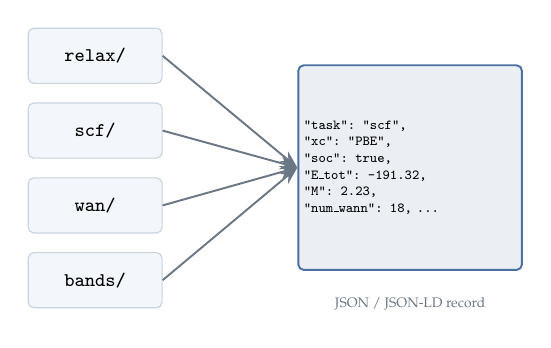
\begin{tikzpicture}[font=\fbook\scriptsize]
  \foreach \i/\n in {0/relax, 1/scf, 2/wan, 3/bands} {
    \node[draw=rule, fill=soft, rounded corners=2pt, minimum width=17mm, minimum height=7mm] (f\i) at (0,-\i*0.95) {\texttt{\n/}};
  }
  \node[box=merged, text width=27mm, minimum height=26mm, align=left, font=\ttfamily\tiny] (rec) at (4.0,-1.42)
   {"task": "scf",\\ "xc": "PBE",\\ "soc": true,\\ "E\_tot": -191.32,\\ "M": 2.23,\\ "num\_wann": 18, \dots};
  \foreach \i in {0,...,3} \draw[arr=muted] (f\i.east) -- (rec.west);
  \node[font=\fbook\tiny, text=muted] at (4.0,-3.15) {JSON / JSON-LD record};
\end{tikzpicture}
\end{column}
\end{columns}
\end{frame}

\begin{frame}{Two readers, complementary failures}
\begin{columns}[T]
\begin{column}{0.47\textwidth}
\begin{plainbox}
{\fsemi\color{parser} Rule-based parser \(\Pars\)}\\[2pt]
\small
\textcolor{good}{\(+\)} exact numbers, fast, any file size\\
\textcolor{good}{\(+\)} deterministic and testable\\
\textcolor{bad}{\(-\)} brittle: only what it was written for\\
\textcolor{bad}{\(-\)} blind to defaults and conventions it does not know
\end{plainbox}
\end{column}
\begin{column}{0.47\textwidth}
\begin{plainbox}
{\fsemi\color{llm} Language model \(\Model\)}\\[2pt]
\small
\textcolor{good}{\(+\)} reads any format, knows code conventions\\
\textcolor{good}{\(+\)} fills gaps (functional from a POTCAR line)\\
\textcolor{bad}{\(-\)} can misread or invent numbers\\
\textcolor{bad}{\(-\)} limited context: cannot read a 500\,MB OUTCAR
\end{plainbox}
\end{column}
\end{columns}
\vspace{4mm}
\begin{keyline}
\textbf{Idea.} Let both read the same files \emph{independently} and \textbf{compare}. Where they agree, confidence is high; where they
disagree, a human looks. Where there is no parser, make the model \textbf{cite its source line} and check it.
\end{keyline}
\end{frame}

\begin{frame}{The pipeline}
\centering
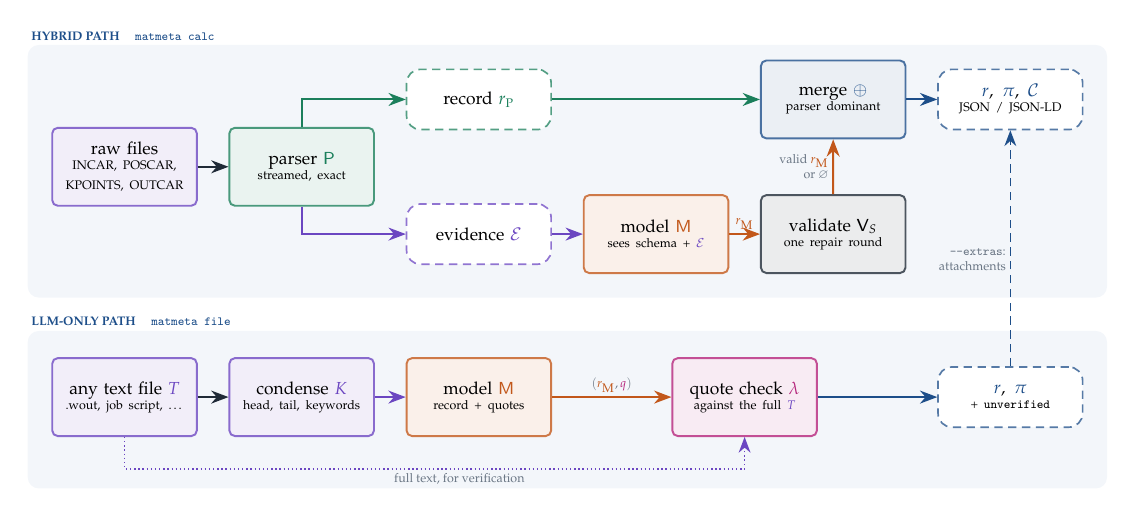
\begin{tikzpicture}[scale=0.9, transform shape, box/.append style={text width=19mm}, data/.append style={text width=19mm}]
  \node[box=evid]   (files) at (0,0)        {raw files\\[-2pt]{\tiny INCAR, POSCAR, KPOINTS, OUTCAR}};
  \node[box=parser] (pars)  at (2.5,0)     {parser \(\Pars\)\\[-2pt]{\tiny streamed, exact}};
  \node[data=parser](rp)    at (5.0,0.95)    {record \(\rP\)};
  \node[data=evid]  (ev)    at (5.0,-0.95)   {evidence \(\Ev\)};
  \node[box=llm]    (mod)   at (7.5,-0.95)  {model \(\Model\)\\[-2pt]{\tiny sees schema + \(\Ev\)}};
  \node[box=ink]    (val)   at (10.0,-0.95)  {validate \(\valid_S\)\\[-2pt]{\tiny one repair round}};
  \node[box=merged] (mer)   at (10.0,0.95)   {merge \(\Merge\)\\[-2pt]{\tiny parser dominant}};
  \node[data=merged](out)   at (12.5,0.95)  {\(\rF,\ \Prov,\ \Conf\)\\[-2pt]{\tiny JSON / JSON-LD}};
  \draw[arr=ink]    (files) -- (pars);
  \draw[arr=parser] (pars.north) |- (rp.west);
  \draw[arr=evid]   (pars.south) |- (ev.west);
  \draw[arr=evid]   (ev) -- (mod);
  \draw[arr=llm]    (mod) -- node[lab, above]{\(\rM\)} (val);
  \draw[arr=parser] (rp) -- (mer);
  \draw[arr=llm]    (val) -- node[lab, left, align=right]{valid \(\rM\)\\or \(\nil\)} (mer);
  \draw[arr=merged] (mer) -- (out);
  \node[box=evid]   (tf)    at (0,-3.25)     {any text file \(\Src\)\\[-2pt]{\tiny .wout, job script, \dots}};
  \node[box=evid]   (cond)  at (2.5,-3.25)  {condense \(\Kop\)\\[-2pt]{\tiny head, tail, keywords}};
  \node[box=llm]    (mod2)  at (5.0,-3.25)   {model \(\Model\)\\[-2pt]{\tiny record + quotes}};
  \node[box=quote]  (chk)   at (8.75,-3.25)   {quote check \(\lam\)\\[-2pt]{\tiny against the full \(\Src\)}};
  \node[data=merged](out2)  at (12.5,-3.25) {\(\rF,\ \Prov\)\\[-2pt]{\tiny + \texttt{unverified}}};
  \draw[arr=ink]    (tf) -- (cond);
  \draw[arr=evid]   (cond) -- (mod2);
  \draw[arr=llm]    (mod2) -- node[lab, above]{\((\rM,\Qt)\)} (chk);
  \draw[arr=merged] (chk) -- (out2);
  \draw[->, >={Stealth[length=2mm]}, evid, line width=0.5pt, densely dotted] (tf.south) -- ++(0,-0.45) -| node[lab, pos=0.27, below]{full text, for verification} (chk.south);
  \draw[->, >={Stealth[length=2mm]}, merged, line width=0.6pt, densely dashed] (out2.north) -- node[lab, left, align=right, pos=0.45]{\texttt{--extras}:\\attachments} (out.south);
  \begin{scope}[on background layer]
    \node[fit=(files)(rp)(ev)(out)(val), inner xsep=3mm, inner ysep=3mm, rounded corners=4pt, fill=soft] (bg1) {};
    \node[fit=(tf)(out2)(chk), inner xsep=3mm, inner ysep=3mm, yshift=-1.6mm, minimum height=20mm, rounded corners=4pt, fill=soft] (bg2) {};
  \end{scope}
  \node[anchor=south west, font=\fbook\tiny\bfseries, text=accent, inner sep=1.5pt] at (bg1.north west) {HYBRID PATH \quad\mdseries\texttt{matmeta calc}};
  \node[anchor=south west, font=\fbook\tiny\bfseries, text=accent, inner sep=1.5pt] at (bg2.north west) {LLM-ONLY PATH \quad\mdseries\texttt{matmeta file}};
\end{tikzpicture}
\end{frame}

% ================================================================ 2
\section{Records, schemas and the parser}

\begin{frame}{Records and schemas}
\begin{defbox}{Record}
A schema \(S\) defines field paths \(\Fset_S\) (\code{results.total\_energy\_eV}, \code{method.task}, \dots) and value types \(\Vset_f\).
A record is a map
\[
  r:\ \Fset_S\to\textstyle\bigcup_f\Vset_f\cup\{\bot\},\qquad \bot=\text{\emph{not stated}} \;(\texttt{null}),\qquad \nil(f)=\bot\ \ \forall f .
\]
\end{defbox}
\begin{columns}[T]
\begin{column}{0.5\textwidth}
\small
\begin{itemize}
\item JSON Schema 2020-12, every leaf nullable, no extra keys.
\item Validation \(\valid_S(x)=\) set of errors; \(\valid_S(x)=\varnothing\iff x\) conforms.
\item Four record types: \code{calculation}, \code{wannier}, \code{jobscript}, \code{abstract}.
\end{itemize}
\end{column}
\begin{column}{0.46\textwidth}
\begin{warnbox}{Conventions live in the schema}
\footnotesize
Descriptions are sent to the model, so notation does not create fake conflicts:\\[1pt]
\textbullet\ formula of the \emph{full cell}: \(\mathrm{Fe_2}\), \(\mathrm{Cu_4In_4P_8S_{24}}\)\\
\textbullet\ standard functional names: \code{GGA=PE} \(\to\) PBE
\end{warnbox}
\end{column}
\end{columns}
\end{frame}

\begin{frame}{Parser: streaming and effective parameters}
\begin{columns}[T]
\begin{column}{0.46\textwidth}
{\fsemi\color{accent} One pass, constant memory}
\small
\begin{itemize}
\item Output read line by line; bounded queues keep the last \(k\le2\) matches.
\[
 \text{time}=O(n),\qquad \text{memory}=O(1)
\]
\item \code{OUTCAR.gz} read transparently \(\Rightarrow\) a multi-GB MD OUTCAR costs nothing extra.
\end{itemize}
\end{column}
\begin{column}{0.5\textwidth}
{\fsemi\color{accent} Which tags did VASP really use?}
\footnotesize

INCAR tags \(\tau_{\mathrm I}\); parameters VASP echoes in the OUTCAR \(\tau_{\mathrm O}\) (defaults included):
\[
 (\tau_{\mathrm O}\Over\tau_{\mathrm I})(k)=\begin{cases}\tau_{\mathrm I}(k) & k\in\operatorname{dom}\tau_{\mathrm I}\\ \tau_{\mathrm O}(k) & \text{otherwise}\end{cases}
\]
and \(\tau=\tau_{\mathrm O}\Over\tau_{\mathrm I}\): explicit INCAR wins; every omitted tag comes from what VASP reports.
\end{column}
\end{columns}
\vspace{3mm}
\begin{keyline}\footnotesize
Harvested: \vtag{IBRION} \vtag{NSW} \vtag{ISIF} \vtag{ISPIN} \vtag{ICHARG} \vtag{ISMEAR} \vtag{SIGMA} \vtag{ENCUT} \vtag{EDIFF}
\vtag{LSORBIT} \vtag{LNONCOLLINEAR} \vtag{LDAU} \vtag{IVDW} \vtag{GGA} \vtag{LEXCH} \vtag{METAGGA} \vtag{LHFCALC} \vtag{HFSCREEN} \vtag{LWANNIER90}
\end{keyline}
\end{frame}

\begin{frame}{Task and functional follow VASP's own rules}
\begin{columns}[T]
\begin{column}{0.5\textwidth}
{\fsemi\color{accent} Task}\\[1pt]
\footnotesize
Defaults when absent: \(\mathrm{NSW}=0\);\ \(\mathrm{IBRION}=-1\) if \(\mathrm{NSW}\in\{0,-1\}\), else \(0\).
\[
\mathrm{task}(\tau)=\begin{cases}
\texttt{nscf} & \vtag{ICHARG}=11\\
\texttt{scf} & \mathrm{IBRION}=-1 \ \text{or}\ \mathrm{NSW}=0\\
\texttt{vc-relax} & \mathrm{IBRION}\in\{1,2,3\},\ \vtag{ISIF}\in\{3,6,7\}\\
\texttt{relax} & \mathrm{IBRION}\in\{1,2,3\}\\
\texttt{md} & \mathrm{IBRION}=0\\
\texttt{phonon} & \mathrm{IBRION}\in\{5,\dots,8\}
\end{cases}
\]
\end{column}
\begin{column}{0.46\textwidth}
{\fsemi\color{accent} Exchange--correlation}\\[1pt]
\footnotesize
\[
\mathrm{xc}(\tau)=\begin{cases}
\tau(\vtag{METAGGA}) & \text{if set}\\
\text{HSE06} & \vtag{LHFCALC},\ \mu=0.2\\
g\bigl(\tau(\vtag{GGA})\bigr) & \vtag{GGA}\neq\texttt{--}\\
g\bigl(\tau(\vtag{LEXCH})\bigr) & \text{otherwise}
\end{cases}
\]
\(g\): \texttt{PE}\(\to\)PBE, \texttt{PS}\(\to\)PBEsol, \texttt{RP}\(\to\)rPBE, \texttt{CA}\(\to\)LDA
\end{column}
\end{columns}
\vspace{2mm}
\begin{warnbox}{Found on a real run}
\footnotesize
Static Wannier90 run on bilayer CuInP\(_2\)S\(_6\), no \vtag{IBRION}, no \vtag{GGA} in the INCAR. v0.1 left both to the model, which said
\textcolor{bad}{\texttt{relax}}. With \(\tau=\tau_{\mathrm O}\Over\tau_{\mathrm I}\) the parser gives \textcolor{good}{\texttt{scf}} and \textcolor{good}{PBE} (\code{LEXCH = PE}).
\end{warnbox}
\end{frame}

\begin{frame}{Energies, moments, structure}
\begin{columns}[T]
\begin{column}{0.48\textwidth}
{\fsemi\color{accent} Energies}
\small

\(F\) = last free energy \code{TOTEN}, \(E_0\) = energy without entropy:
\[
 E_{\sigma\to0}=\tfrac12\,(F+E_0)
\]
Both are stored: \code{total\_energy\_eV}\(=F\), \code{energy\_sigma0\_eV}\(=E_{\sigma\to0}\).
For metals with large \(\sigma\), compare \(E_{\sigma\to0}\).

\vspace{2mm}
{\fsemi\color{accent} Structure}

CONTCAR (final geometry) for \texttt{relax}, \texttt{vc-relax}, \texttt{md}; else POSCAR. Recorded in \code{structure\_from}.
\end{column}
\begin{column}{0.48\textwidth}
{\fsemi\color{accent} Magnetic moment}
\small
Collinear: \(M_{\mathrm{tot}}=m\).\quad Noncollinear:
\[
M_{\mathrm{tot}}=\lVert\mathbf m\rVert=\sqrt{m_x^2+m_y^2+m_z^2},
\]
and the vector \(\mathbf m=(m_x,m_y,m_z)\) is stored too.
\vspace{2mm}
\begin{warnbox}{v0.1 bug, now fixed}
\footnotesize
Only \(m_x\) was read in noncollinear runs: a moment along \(z\) was reported as \(\approx 10^{-6}\,\mu_{\mathrm B}\).
\end{warnbox}
\end{column}
\end{columns}
\end{frame}

\begin{frame}{What the model sees: the evidence text}
\begin{columns}[T]
\begin{column}{0.48\textwidth}
\small
\begin{itemize}
\item INCAR \textbf{verbatim}
\item KPOINTS, first six lines
\item POSCAR/CONTCAR header \textbf{verbatim}
\item OUTCAR: version, POTCAR lines, the parameter block, last \(F\), \(E_{\sigma\to0}\), \(E_{\mathrm F}\), moments, convergence message
\end{itemize}
\muted{\footnotesize A few dozen lines, independent of the OUTCAR size.}
\end{column}
\begin{column}{0.48\textwidth}
\begin{warnbox}{An honest caveat}
\footnotesize
Split the fields: \(\Fset=\Fset_{\mathrm{in}}\sqcup\Fset_{\mathrm{out}}\).\\[2pt]
\(\Fset_{\mathrm{in}}\) (settings) are read by the model from \emph{verbatim} input: agreement \(\rM(f)\agree\rP(f)\) validates the parser's \emph{interpretation}.\\[2pt]
\(\Fset_{\mathrm{out}}\) (energies, moments) come from lines the \emph{parser selected}: agreement confirms the reading of the line, not the choice of the line.
\end{warnbox}
\end{column}
\end{columns}
\end{frame}

% ================================================================ 3
\section{The model and the merge}

\begin{frame}{Schema-constrained query with one repair round}
\begin{columns}[T]
\begin{column}{0.5\textwidth}
\begin{plainbox}
\small
\(y\leftarrow\Model(\sigma,\ \mathrm{prompt}(S,\Ev))\)\\
\(e\leftarrow\valid_S(y)\)\\
\textbf{if} \(e\neq\varnothing\):\\
\quad \(y\leftarrow\Model(\sigma,\ \mathrm{prompt}(S,\Ev,\textcolor{bad}{e}))\)\\
\quad \(e\leftarrow\valid_S(y)\)\\
\textbf{return} \((y,e)\)
\end{plainbox}
\small
Temperature 0; JSON requested; code fences and chatter tolerated.
\end{column}
\begin{column}{0.46\textwidth}
\[
\rM=\begin{cases} y & \text{call succeeded and } e=\varnothing\\ \nil & e\neq\varnothing \text{ or the call raised}\end{cases}
\]
\begin{propbox}{Safe failure}
\footnotesize
Server down, wrong key, timeout, garbage reply \(\Rightarrow \rM=\nil\Rightarrow\rF=\rP\).
The run still produces a record; the error is kept in \code{llm\_error}. Batch jobs never lose a folder.
\end{propbox}
\end{column}
\end{columns}
\end{frame}

\begin{frame}{Agreement and merge}
\begin{columns}[T]
\begin{column}{0.4\textwidth}
\begin{defbox}{Agreement}
\footnotesize
\(a\agree b\) when\\[1pt]
\textbullet\ numbers:
\[|a-b|\le\max\bigl(\rho\max(|a|,|b|),\,\alpha\bigr)\]
\vspace{-2mm}\phantom{\textbullet\ }\(\rho=10^{-3},\ \alpha=10^{-6}\)\\
\textbullet\ strings: trimmed, case-folded\\
\textbullet\ Booleans: identical\\
\textbullet\ arrays: element-wise (lattice vectors)
\end{defbox}
\end{column}
\begin{column}{0.56\textwidth}
\begin{defbox}{Merge}
\footnotesize
\(\rF=\rP\Merge\rM\), field by field:\\[2pt]
\begin{tabular}{@{}lll@{}}
\((\rP(f),\rM(f))\) & \(\rF(f)\) & \(\Prov(f)\)\\\midrule
both set, \(\agree\)    & \(\rP(f)\) & \texttt{parser+llm}\\
both set, \(\nagree\)   & \(\rP(f)\) & \texttt{parser (llm disagreed)}\\
only \(\rP\)            & \(\rP(f)\) & \texttt{parser}\\
only \(\rM\)            & \(\rM(f)\) & \texttt{llm}\\
neither                 & \(\bot\)   & \texttt{missing}
\end{tabular}\\[3pt]
\(\Conf=\{f:\ \Prov(f)=\texttt{parser (llm disagreed)}\}\)
\end{defbox}
\end{column}
\end{columns}
\vspace{1mm}
\begin{propbox}{Properties}
\footnotesize
(i) \(\rP(f)\neq\bot\Rightarrow\rF(f)=\rP(f)\): the model adds, never overwrites. \quad
(ii) \(\rM=\nil\Rightarrow\rF=\rP,\ \Conf=\varnothing\). \quad
(iii) \(\valid_S(\rP)=\valid_S(\rM)=\varnothing\Rightarrow\valid_S(\rF)=\varnothing\). \quad
(iv) independent of field order.
\end{propbox}
\end{frame}

% ================================================================ 4
\section{Files without a parser: quote verification}

\begin{frame}[fragile]{No parser? Make the model cite its line}
\small
For Wannier90 \code{.wout}, job scripts, other codes' output, in-house logs:
\[
 \Model(\sigma_{\mathrm q},\,\Kop(\Src))\ \longmapsto\ (\rM,\ \Qt),\qquad \Qt:\ f\mapsto\text{the source line of } \rM(f)
\]
\begin{columns}[T]
\begin{column}{0.5\textwidth}
\begin{defbox}{Checks against the full file}
\footnotesize
\(\norm\): collapse white space.\\[3pt]
\(\mathsf{found}(\Qt_f)\iff\norm(\Qt_f)\subseteq\norm(\Src)\)\\[3pt]
\(\mathsf{contains}(v,\Qt_f)\): \\
\textbullet\ number: \(\exists\,n\in\Nums(\Qt_f),\ c\in\mathcal U:\ c\,n\approx v\) to \(10^{-4}\)\\
\textbullet\ string or alias in the line; arrays element-wise\\[2pt]
\(\mathcal U=\{1,\mathrm{Ry},\mathrm{Ha},a_0,a_0^2,\mathrm{Ry}^{-1}\}\)
\end{defbox}
\end{column}
\begin{column}{0.46\textwidth}
\begin{lstlisting}
"record": {"wannierisation":
   {"omega_total_A2": 33.10213342}},
"quotes": {"wannierisation.omega_total_A2":
   "Final Spread (Ang^2)  Omega Total
                      =  33.102133420"}
\end{lstlisting}
\vspace{-1mm}
{\footnotesize\textcolor{good}{\(\checkmark\)} line found, number on it \(\Rightarrow\) \texttt{llm (verified)}}
\end{column}
\end{columns}
\end{frame}

\begin{frame}{Labels and strict mode}
\begin{columns}[T]
\begin{column}{0.6\textwidth}
\footnotesize
\[
\lam(f)=\begin{cases}
\texttt{missing} & v=\bot\\
\textcolor{bad}{\texttt{unverified: no quote}} & \Qt_f \text{ absent}\\
\textcolor{bad}{\texttt{unverified: quote not in file}} & \neg\mathsf{found}\\
\texttt{quote found} & v \text{ Boolean}\\
\textcolor{good}{\texttt{verified}} & \mathsf{found}\wedge\mathsf{contains}\\
\textcolor{bad}{\texttt{unverified: value not in quote}} & \text{otherwise}
\end{cases}
\]
\end{column}
\begin{column}{0.37\textwidth}
\begin{plainbox}
\footnotesize
\textbf{Default:} keep the value, list the field in \code{unverified}, print \code{[unverified]}.\\[3pt]
\textbf{\texttt{--strict}:} set \(\rF(f)=\bot\), label \texttt{dropped (\dots)}.
\end{plainbox}
\begin{plainbox}
\footnotesize
Aliases for named values: \texttt{slurm} accepted if the line has \code{\#SBATCH} or \code{srun}.
\end{plainbox}
\end{column}
\end{columns}
\end{frame}

\begin{frame}{What the quote check can and cannot catch}
\begin{columns}[T]
\begin{column}{0.48\textwidth}
\begin{propbox}{Caught}
\small
\textbullet\ an invented number with no quote\\
\textbullet\ an invented line that is not in the file\\
\textbullet\ a real line paired with a number that is not on it\\[3pt]
\muted{\footnotesize The common failure modes of small local models.}
\end{propbox}
\end{column}
\begin{column}{0.48\textwidth}
\begin{warnbox}{Not caught}
\small
\textbullet\ misattribution: the number is on the line but belongs to another quantity (\(\Omega_{\mathrm D}\) reported as \(\Omega_{\mathrm{tot}}\))\\
\textbullet\ a line from the wrong iteration of a repeated block\\
\textbullet\ Booleans: only the line's existence is checked
\end{warnbox}
\end{column}
\end{columns}
\vspace{3mm}
\begin{keyline}\small
A strong filter for \emph{fabrication}, not a proof of \emph{correctness}. Next step: physical consistency checks, e.g.
\(\Omega=\Omega_{\mathrm I}+\Omega_{\mathrm D}+\Omega_{\mathrm{OD}}\), which catch exactly the misattributions.
\end{keyline}
\end{frame}

\begin{frame}{Condensing long files}
\begin{columns}[T]
\begin{column}{0.62\textwidth}
\footnotesize
Lines \(0,\dots,n-1\); keyword hits \(H\) (at most \(h_{\max}\)):
\[
\Kop(\Src)=\begin{cases}\Src & |\Src|\le L\\
\Src\big|_I,\ \ I=[0,h)\cup[n-t,n)\cup\textstyle\bigcup_{i\in H}[i-c,i+c] & \text{else}\end{cases}
\]
Gaps become \code{[... k lines skipped ...]}.\\[2pt]
\(L=24\,000\) chars, \(h=80\), \(t=150\), \(c=1\), \(h_{\max}=300\).
\end{column}
\begin{column}{0.34\textwidth}
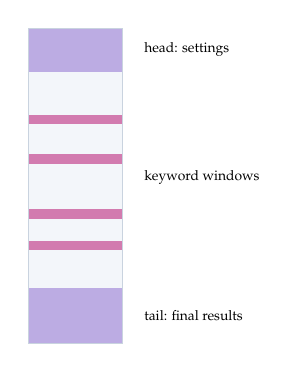
\begin{tikzpicture}[font=\fbook\tiny]
  \fill[soft] (0,0) rectangle (1.2,-4.0);
  \fill[evid!45] (0,0) rectangle (1.2,-0.55);
  \fill[evid!45] (0,-3.3) rectangle (1.2,-4.0);
  \foreach \y in {-1.1,-1.6,-2.3,-2.7} \fill[quote!60] (0,\y) rectangle (1.2,\y-0.12);
  \draw[rule] (0,0) rectangle (1.2,-4.0);
  \node[anchor=west] at (1.35,-0.27) {head: settings};
  \node[anchor=west] at (1.35,-1.9) {keyword windows};
  \node[anchor=west] at (1.35,-3.65) {tail: final results};
\end{tikzpicture}
\end{column}
\end{columns}
\vspace{2mm}
\begin{propbox}{Why it is safe}
\footnotesize
\(\lam\) is evaluated against the \emph{full} \(\Src\): condensation can make a value \texttt{missing}, never make a fabricated one pass.
\end{propbox}
\end{frame}

% ================================================================ 5
\section{Composite records and JSON-LD}

\begin{frame}{New record types}
\begin{columns}[T]
\begin{column}{0.48\textwidth}
\begin{plainbox}
{\fsemi\color{accent}\small Wannier90 \code{.wout}}\\[1pt]
\footnotesize
release, \code{num\_wann}, \code{num\_bands}, MP grid, spinors\\
outer / frozen windows (eV), disentanglement convergence, \(\Omega_{\mathrm I}\)\\
wannierisation convergence, \(\Omega_{\mathrm I},\Omega_{\mathrm D},\Omega_{\mathrm{OD}},\Omega\) (\AA\(^2\))
\end{plainbox}
\end{column}
\begin{column}{0.48\textwidth}
\begin{plainbox}
{\fsemi\color{accent}\small Batch job script}\\[1pt]
\footnotesize
scheduler, partition, nodes, tasks, CPUs, GPUs, memory, time limit, constraint\\
loaded modules, executable, launcher\\
\muted{\code{vasp\_ncl} independently confirms a noncollinear build}
\end{plainbox}
\end{column}
\end{columns}
\vspace{2mm}
\small Detected automatically: suffix \code{.wout}; scripts with \code{\#SBATCH}, \code{\#PBS}, \code{\#BSUB}, \code{\#\$}, or a shebang plus \code{srun}/\code{mpirun}.
\end{frame}

\begin{frame}[fragile]{One record per run folder}
\begin{columns}[T]
\begin{column}{0.5\textwidth}
\small
With \code{--extras}, a run directory \(D\) gives
\[
R(D)=\bigl(\rF_{\mathrm{calc}},\Prov,\Conf,\ \{(\phi,\kappa_\phi,\rF_\phi,\Prov_\phi)\}_{\phi\in X(D)}\bigr)
\]
\(X(D)\): the \code{.wout} files and job scripts found in \(D\).
\vspace{2mm}

JSON-LD export: field \(\mapsto\) ontology term via \code{@context}; nulls dropped; units as \(\{\texttt{value},\texttt{unit}\}\);
attachments as \code{hasPart}.
\end{column}
\begin{column}{0.46\textwidth}
\begin{lstlisting}
{ "@type": "mm:DFTCalculation",
  "method": {"xc_functional": "PBE",
             "spin_orbit_coupling": true},
  "attachments": [
   { "@type": "mm:Wannier90Run",
     "wannierisation": {"omega_total_A2":
        {"value": 33.102,
         "unit": "square angstrom"}}},
   { "@type": "mm:BatchJob",
     "software": {"executable":
                  "vasp_ncl"}} ] }
\end{lstlisting}
\end{column}
\end{columns}
\end{frame}

% ================================================================ 6
\section{Results on real calculations}

\begin{frame}{Test 1: bcc Fe with llama3.1 (8B, local, Ollama)}
\begin{columns}[T]
\begin{column}{0.46\textwidth}
\small
\begin{itemize}
\item \textcolor{good}{\fbook 16 fields} \texttt{parser+llm}: energy, \(E_{\mathrm F}\), moment, ENCUT, k-mesh, smearing, version, lattice \dots
\item 3 fields filled by the model only (DFT+U, SOC, noncollinear: tags absent from the INCAR, so no cross-check)
\item \textcolor{llm}{\fbook 2 conflicts}, both caught:
\end{itemize}
\end{column}
\begin{column}{0.5\textwidth}
\footnotesize
\begin{tabular}{@{}lll@{}}
\toprule
field & \textcolor{parser}{parser} & \textcolor{llm}{llama3.1}\\\midrule
\code{formula} & Fe2 & Fe \\
\code{xc\_functional} & PBE & PE \\
\bottomrule
\end{tabular}
\vspace{2mm}

\textbullet\ reduced vs full-cell formula: a \emph{notation} conflict\\
\textbullet\ raw tag copied: \code{GGA = PE}\\[2pt]
\(\Rightarrow\) both fixed by schema conventions in v0.2; the parser's value was kept in both cases.
\end{column}
\end{columns}
\end{frame}

\begin{frame}{Test 2: bilayer CuInP\(_2\)S\(_6\), PBE+SOC+D3, Wannier90 run}
\begin{columns}[T]
\begin{column}{0.5\textwidth}
\footnotesize
\begin{tabular}{@{}ll@{}}
\toprule
\multicolumn{2}{@{}l}{\fbook extracted record}\\\midrule
formula & Cu\(_4\)In\(_4\)P\(_8\)S\(_{24}\) (40 atoms, \(c\approx53\)\,\AA)\\
method & SOC, noncollinear, IVDW=12 (D3-BJ)\\
numerics & 500 eV, \(5\times4\times1\), Gaussian 0.05 eV\\
results & \(F=-191.320\) eV, \(E_{\mathrm F}=-3.141\) eV\\
xc & PBE \textcolor{llm}{(model, from POTCAR)}\\
\bottomrule
\end{tabular}
\end{column}
\begin{column}{0.46\textwidth}
\footnotesize
\begin{tabular}{@{}lll@{}}
\toprule
field & \textcolor{parser}{v0.1 parser} & \textcolor{llm}{llama3.1}\\\midrule
smearing & Gaussian & \textcolor{bad}{FERDO} \\
task & \(\bot\) & \textcolor{bad}{relax} \\
\bottomrule
\end{tabular}
\vspace{2mm}

\textbullet\ \texttt{FERDO}: caught as a conflict, parser kept\\
\textbullet\ \texttt{relax}: \emph{not} caught, because the parser had no value. Found by inspection \(\Rightarrow\) the \(\tau_{\mathrm O}\Over\tau_{\mathrm I}\) rule\\
\textbullet\ the review it prompted also found the \(m_x\)-only moment bug
\end{column}
\end{columns}
\vspace{2mm}
\begin{keyline}\footnotesize
Lesson: fields marked \texttt{llm} carry no cross-check. Moving them to the parser (or to the quote check) is where accuracy is gained.
\end{keyline}
\end{frame}

\begin{frame}{Worked example: v0.1 vs v0.2 on \code{examples/vasp\_Fe\_soc}}
\centering\small
\begin{tabular}{@{}llll@{}}
\toprule
field & v0.1 & v0.2 & rule \\\midrule
\code{task} & \textcolor{bad}{\(\bot\)} & \textcolor{good}{scf} & \vtag{IBRION}\(=-1\) from \(\tau_{\mathrm O}\)\\
\code{xc\_functional} & \textcolor{bad}{\(\bot\)} & \textcolor{good}{PBE} & no \vtag{GGA}; \vtag{LEXCH}\(=\)\texttt{PE}\\
\code{total\_magnetization\_muB} & \textcolor{bad}{\(1.1\times10^{-6}\)} & \textcolor{good}{2.231} & \(\lVert\mathbf m\rVert\)\\
\code{magnetization\_vector\_muB} & --- & \((0,0,2.231)\) & three components\\
\code{energy\_sigma0\_eV} & --- & \(-8.29514\) & \(\tfrac12(F+E_0)\)\\
attachments & --- & \code{wannier90.wout}, \code{z\_jobs\_ibex} & \code{--extras}\\
\bottomrule
\end{tabular}
\vspace{4mm}

\begin{keyline}\footnotesize
\(\Omega_{\mathrm I}+\Omega_{\mathrm D}+\Omega_{\mathrm{OD}} = 31.250048+0.004512+1.847573 = 33.102133\ \text{\AA}^2=\Omega\)\quad\muted{(consistent record)}
\end{keyline}
\end{frame}

% ================================================================ 7
\section{Using it, metrics and roadmap}

\begin{frame}[fragile]{Using it}
\begin{columns}[T]
\begin{column}{0.55\textwidth}
\begin{lstlisting}
# local model, data never leaves the machine
export MATMETA_BASE_URL=http://localhost:11434/v1
export MATMETA_MODEL=llama3.1

matmeta calc .  --no-llm         # parser only
matmeta calc .  --extras         # + .wout, job script
matmeta calc runs/*/ --jsonld -o metadata/
matmeta file wannier90.wout --strict
matmeta abstract abstract.txt
\end{lstlisting}
\end{column}
\begin{column}{0.41\textwidth}
\small
Diagnostics on stderr:\\[2pt]
\footnotesize
\begin{tabular}{@{}ll@{}}
\code{[conflict]} & parser \(\nagree\) model\\
\code{[unverified]} & quote check failed\\
\code{[warning]} & model down / invalid\\
\code{[error]} & unreadable input
\end{tabular}
\vspace{3mm}

\small
Any OpenAI-compatible server: Ollama, vLLM on an HPC GPU node, or a hosted API.\\[2pt]
\muted{\footnotesize 31 offline tests, Python 3.9--3.13.}
\end{column}
\end{columns}
\end{frame}

\begin{frame}{How to measure it}
\small
For gold records \(r^\ast\) on a curated set of runs, per field \(f\):
\[
\mathrm{precision}_f=\frac{\#\{\rF(f)\neq\bot,\ \rF(f)\agree r^\ast(f)\}}{\#\{\rF(f)\neq\bot\}},
\qquad
\mathrm{recall}_f=\frac{\#\{\rF(f)\neq\bot,\ \rF(f)\agree r^\ast(f)\}}{\#\{r^\ast(f)\neq\bot\}}
\]
\begin{columns}[T]
\begin{column}{0.48\textwidth}
\begin{itemize}
\item split by provenance class: \texttt{parser+llm}, \texttt{parser}, \texttt{llm}
\item conflict rate \(|\Conf|/|\Fset|\)
\end{itemize}
\end{column}
\begin{column}{0.48\textwidth}
\begin{itemize}
\item LLM-only path: verification rate and precision of \texttt{verified} values
\item compare local 7--8\,B vs larger hosted models
\end{itemize}
\end{column}
\end{columns}
\end{frame}

\begin{frame}{Roadmap}
\begin{columns}[T]
\begin{column}{0.48\textwidth}
\begin{itemize}
\item \textbf{Consistency constraints} on records: \(\Omega\) decomposition, \(n_{\mathrm{atoms}}=\sum_s n_s\), \(N_{\mathrm{tasks}}=N_{\mathrm{nodes}}N_{\mathrm{tasks/node}}\)
\item \textbf{More parsers} (SIESTA, Wannier90, phonopy, LAMMPS): move codes from the LLM-only to the hybrid path
\end{itemize}
\end{column}
\begin{column}{0.48\textwidth}
\begin{itemize}
\item \textbf{Community ontologies} and export to research-data repositories
\item \textbf{Papers \(\leftrightarrow\) data}: extract from full texts and link each publication to the records of its calculations
\item \textbf{Benchmark} across models with the metrics above
\end{itemize}
\end{column}
\end{columns}
\end{frame}

\begin{frame}{Summary}
\begin{columns}[c]
\begin{column}{0.58\textwidth}
\begin{enumerate}
\item Two independent readers, \(\rP\) and \(\rM\), merged under parser dominance: \(\rF=\rP\Merge\rM\)
\item Every field has a provenance \(\Prov(f)\); disagreements form \(\Conf\)
\item Without a parser, values must cite a source line, checked by \(\lam\) against the full file
\item The model can be down or wrong without corrupting a record
\item Runs locally: unpublished data stays at the institution
\end{enumerate}
\end{column}
\begin{column}{0.38\textwidth}
\begin{plainbox}
\footnotesize
\textbf{Code}\\ github.com/Gokaran-Shukla/llm-matmeta\\[3pt]
\textbf{Formalism}\\ docs/llm-matmeta-formalism.pdf\\[3pt]
\textbf{Cite}\\ doi:10.5281/zenodo.24334736
\end{plainbox}
\end{column}
\end{columns}
\end{frame}

{\setbeamertemplate{footline}{}
\setbeamercolor{background canvas}{bg=accent}
\begin{frame}[plain,noframenumbering]
\centering
\vspace{14mm}
{\color{white}\fthin\fontsize{36}{40}\selectfont Thank you}\\[8mm]
{\color{white!80!accent}\fbook\small gokaran.shukla@kaust.edu.sa \quad\textbullet\quad gokaran-shukla.github.io}
\end{frame}}

\end{document}
